\subsection{Separate Bewegungsabläufe}

Das erste Ziel ist es dem Läufer das stehen bleiben beizubringen. Hierfür soll der Läufer sich möglichst wenig von der aktuellen Position bewegen. Die Hauptaufgabe ist es hierbei das Gleichgewicht zu halten. 

Für das stehenbleiben wird die Zielgeschwindigkeit auf 0 gesetzt während das Ziel auf der Startposition befindet. Die Belohnungsfunktion der Demo, wird ab jetzt Demo Belohnungsfunktion genannt. Die Demo Belohnungsfunktion hat das Problem das durch die Zielgeschwindigkeit geteilt wird, was bei einer Zielgeschwindigkeit von 0 zu Mathematischen Fehlern führt. Um das zu vermeiden wurde das trainieren mit einer anderen Belohnungsfunktion getestet.

\begin{figure}[H]
  \centering  
  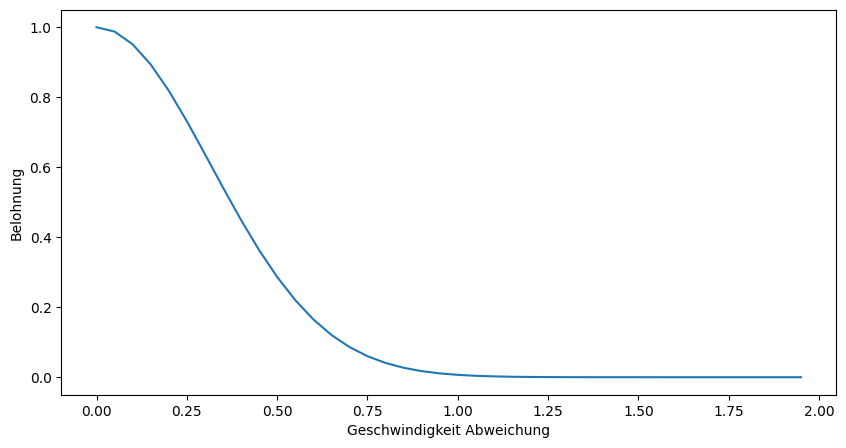
\includegraphics[width=0.9\textwidth]{img/plot_vel_reward_neu}
  \caption{Neue Sigmoid Geschwindigkeit Belohnungsfunktion}
  \label{fig:plot_vel_reward_neu}
\end{figure}

Als neue Belohnungsfunktion wird eine ähnliche Sigmoid Funktion genutzt. Die Belohnungsfunktion nimmt für eine perfekte Übereinstimmung zwischen aktueller Geschwindigkeit und Zielgeschwindigkeit eine Belohnung von 1 an. Mit steigender Abweichung nimmt auch die Belohnung immer weiter ab. Ist eine Abweichung von größer 1 erreicht ist die Belohnung 0. Die Belohnungsfunktion aus Abbildung \ref{fig:plot_vel_reward_neu} wird daher ab hier Neue Belohnungsfunktion genannt.

Der Walker konnte mit der Neuen Belohnungsfunktion lernen auf der Stelle zu stehen.  Abbildung \ref{fig:126_move_target_dir}, \ref{fig:126_episode_length} zeigt wie die zurück gelegte Distanz um 0 herum pendelt, während die Episodenlänge die maximale Länge von 1000 erreicht hat. Die Belohnungen sind auch nahezu maximal ausgereizt siehe Abbildung \ref{fig:126_look_reward}, \ref{fig:126_vel_reward}.

\begin{figure}[H]
  \centering  
  \begin{subfigure}{.49\textwidth}
      \centering  
      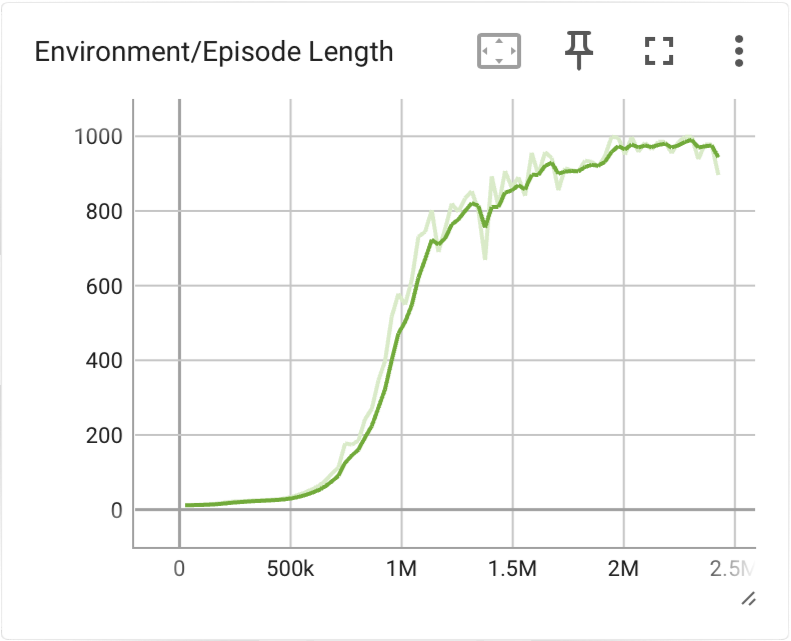
\includegraphics[width=\textwidth]{img/126_episode_length}
      \caption{Episodenlänge}
      \label{fig:126_episode_length}
    \end{subfigure}
    \begin{subfigure}{.49\textwidth}
      \centering  
      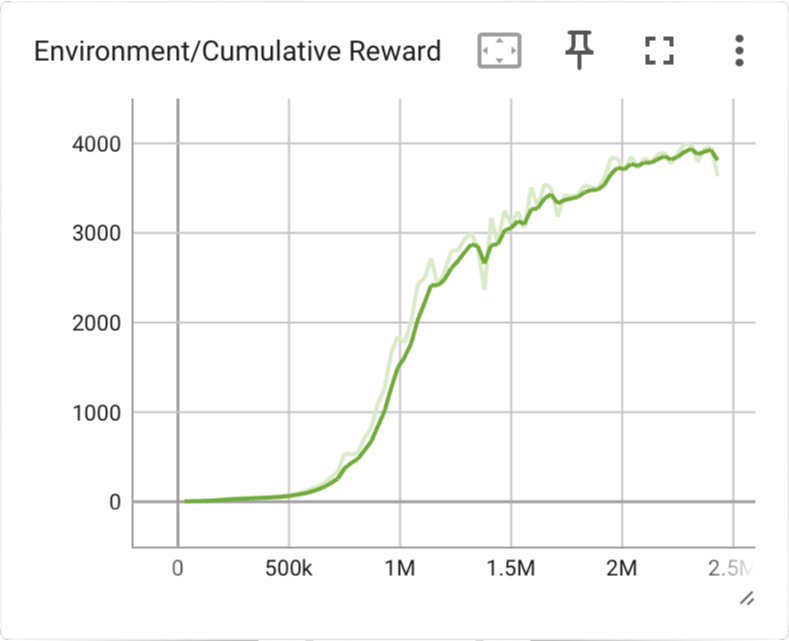
\includegraphics[width=\textwidth]{img/126_cumulative_reward}
      \caption{Angehäufte Belohnung}
      \label{fig:126_cumulative_reward}
    \end{subfigure}
     \begin{subfigure}{.49\textwidth}
      \centering  
      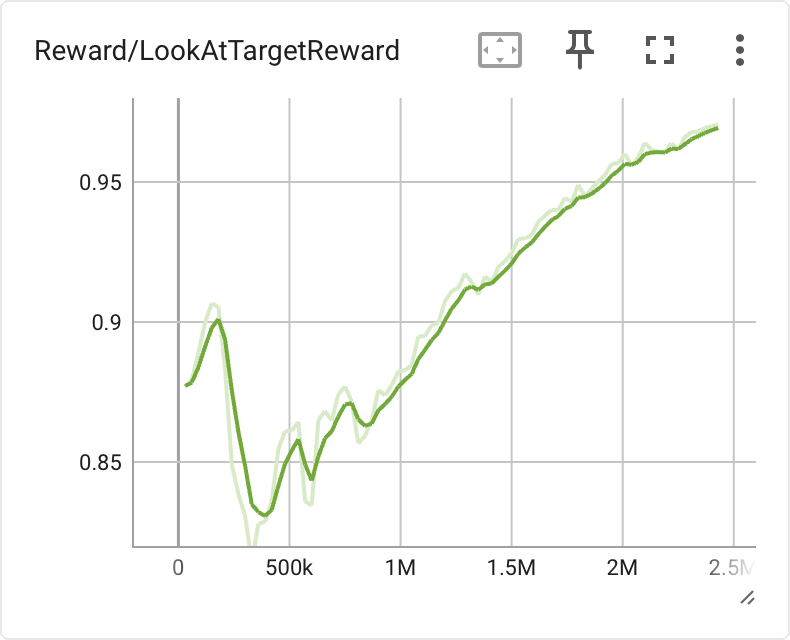
\includegraphics[width=\textwidth]{img/126_look_reward}
      \caption{Blickbelohnung}
      \label{fig:126_look_reward}
    \end{subfigure}
    \begin{subfigure}{.49\textwidth}
      \centering  
      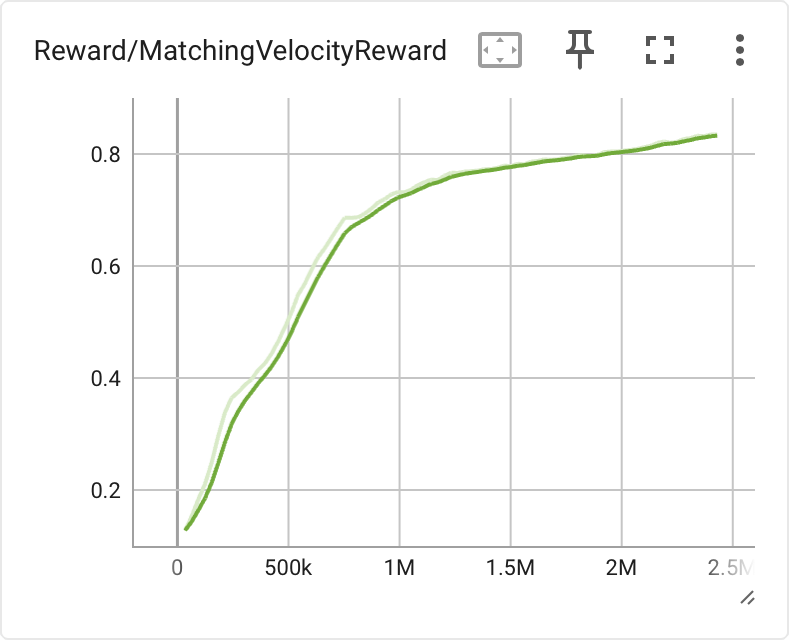
\includegraphics[width=\textwidth]{img/126_vel_reward}
      \caption{Geschwindigkeitsbelohnung}
      \label{fig:126_vel_reward}
    \end{subfigure}
    \begin{subfigure}{.49\textwidth}
      \centering  
      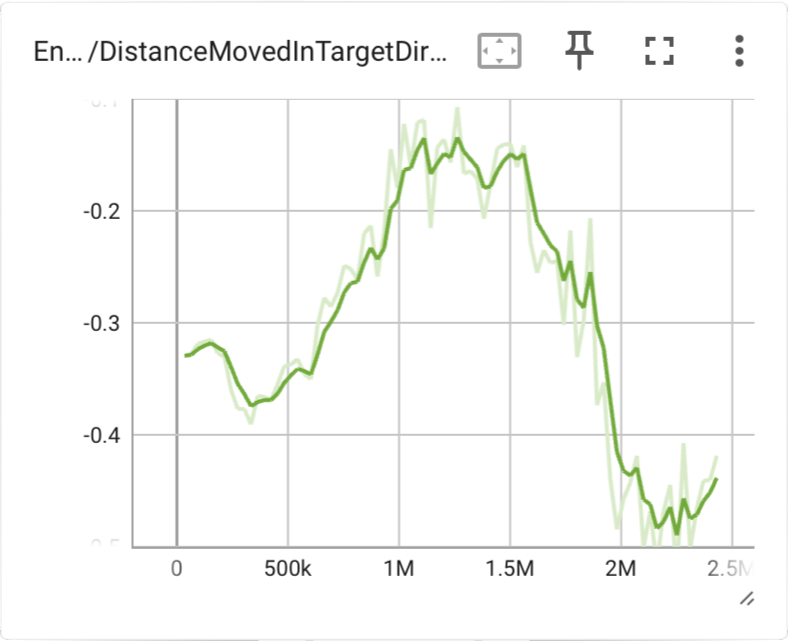
\includegraphics[width=\textwidth]{img/126_move_target_dir}
      \caption{Zurückgelegte Stecke in Zielrichtung}
      \label{fig:126_move_target_dir}
    \end{subfigure}
  \caption{Training Stehen mit neuer Belohnungsfunktion}
  \label{fig:training_stehen_neu}
\end{figure}

Mit zufälliger Zielgeschwindigkeit zu einem Ziel zu laufen wie im Ursprünglichen Verhalten konnte damit jedoch nicht zufriedenstellend erlernt werden. Die Abbildung \ref{fig:training_vergleich_demo_neu} zeigt mit der orangenen Linie die Leistung der Neuen Belohnungsfunktion und mit der rosa Linie die Leistung der Demo Belohnungsfunktion. Nachfolgender Vergleich der Belohnungsfunktionen zeigt das die Ursprüngliche Belohnungsfunktion durch das Teilen mit der Zielgeschwindigkeit die Sensitivität der Funktion je nach Zielgeschwindigkeit beeinflusst. Daraus folgt das bei steigender Zielgeschwindigkeit eine größere Abweichung der Geschwindigkeit geduldet wird (siehe Abbildung \ref{fig:match_velocity_demo_vergleich}). Diese Anpassung verbessert die Generalisierung zwischen den wechselnden Geschwindigkeiten um ein vielfaches.

\begin{figure}[H]
  \centering  
  \begin{subfigure}{.49\textwidth}
      \centering  
      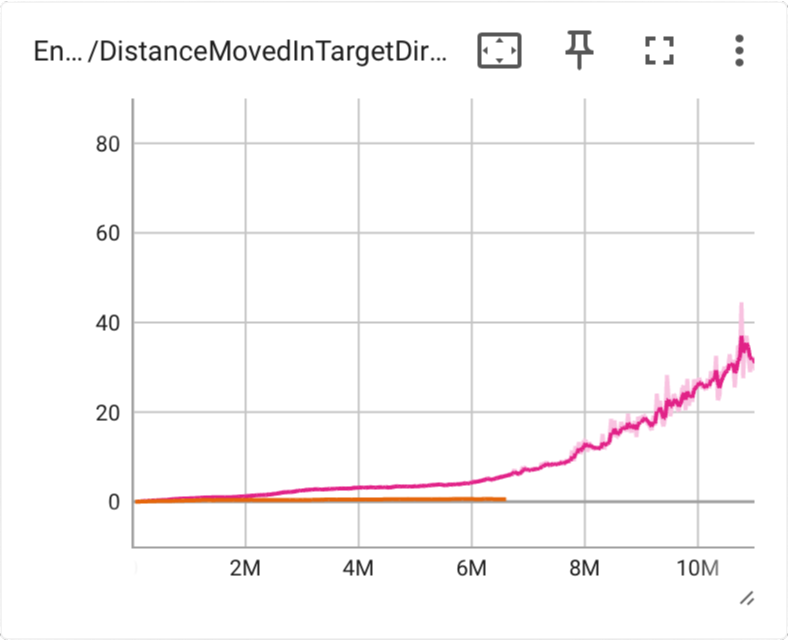
\includegraphics[width=\textwidth]{img/116_127_move_target_dir}
      \caption{Zurückgelegte Stecke in Zielrichtung}
      \label{fig:116_127_move_target_dir}
    \end{subfigure}
    \begin{subfigure}{.49\textwidth}
      \centering  
      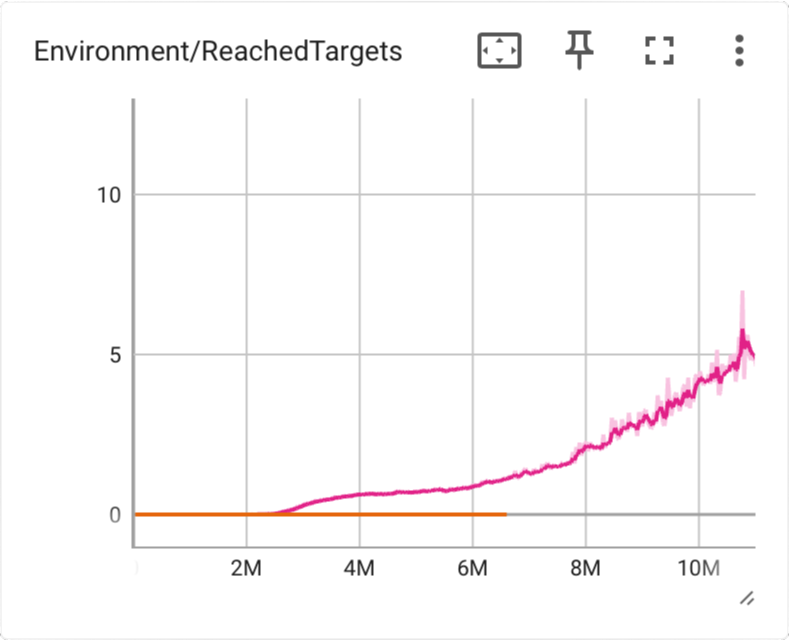
\includegraphics[width=\textwidth]{img/116_127_reach_target}
      \caption{Anzahl erreichte Ziele}
      \label{fig:116_127_reach_target}
    \end{subfigure}
  \caption{Vergleich von Lauftraining mit Demo Belohnungsfunktion gegen Neue Belohnungsfunktion}
  \label{fig:training_vergleich_demo_neu}
\end{figure}

\begin{figure}[H]
  \centering  
  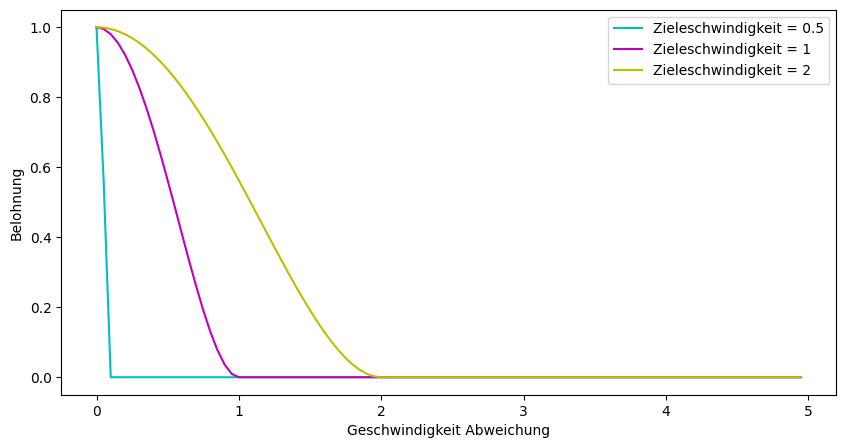
\includegraphics[width=0.9\textwidth]{img/match_velocity_demo_vergleich}
  \caption{Vergleich der Demo Belohnungsfunktion unter verschiedenen Zielgeschwindigkeiten}
  \label{fig:match_velocity_demo_vergleich}
\end{figure}

Mit dieser Erkenntnis aus wird eine neue Anpassung untersucht. In der folgenden Anpassung bleibt die Belohnungsfunktion weitestgehend Unverändert. Lediglich das obere Limit ab welchem die Funktion eine Belohnung von 0 annimmt, wird auf ein minimum von 0.1 beschränkt. Somit kann sichergestellt werden, dass im Bereich der normalen Fortbewegung keine Veränderung auftritt. Mit der Demo Belohnungsfunktion konnten nur Annäherungen an eine Zielgeschwindigkeit von 0 genutzt werden. Bei immer weiterer Annäherung an 0 wird das Spektrum an akzeptablen Geschwindigkeiten bevor die Belohnung 0 ist nahezu unerreichbar (siehe Abbildung \ref{fig:match_velocity_vergleich_clip}). Mit dem Limit von 0.1 ist der Bereich an Abweichungen für die die Belohnungsfunktion einen Wert größer 0 annimmt groß genug. Der Läufer kann durch ausprobieren Belohnungen über 0 erreichen, wodurch eine Richtung für die Optimierung ermittelt werden kann. Somit kann der Läufer die Belohnung optimieren.\\

\begin{figure}[H]
  \centering  
  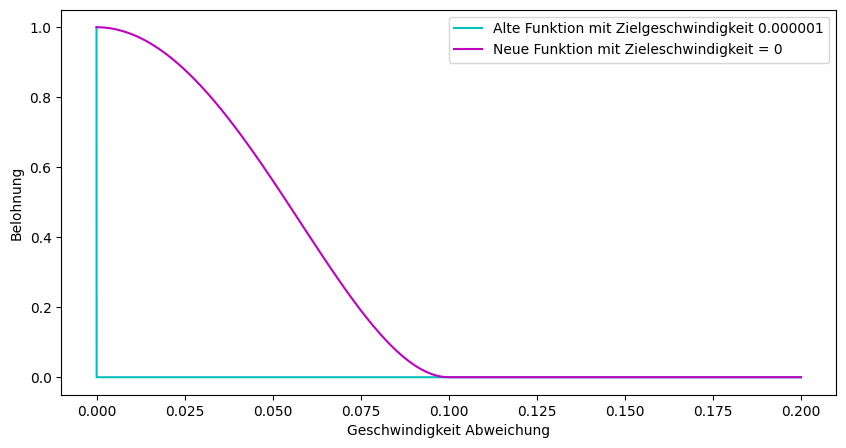
\includegraphics[width=0.9\textwidth]{img/match_velocity_vergleich_clip}
  \caption{Vergleich Demo gegen Belohnungsfunktion mit 0.1 Limit}
  \label{fig:match_velocity_vergleich_clip}
\end{figure}
Das auf einer Stelle stehen hat der Läufer damit in einem separaten Training auch erlernt. Abbildung \ref{fig:128_episode_length} zeigt das der Läufer die maximale Episoden Länge von 1000 erreicht hat ohne zu fallen. Die bewegte Distanz hat sich auch 0 angenähert (siehe \ref{fig:128_move_target_dir}. Die Belohnungen wurden auch weitestgehend optimiert siehe Abbildung \ref{fig:128_look_reward}, \ref{fig:128_vel_reward}.


\begin{figure}[H]
  \centering  
  \begin{subfigure}{.49\textwidth}
      \centering  
      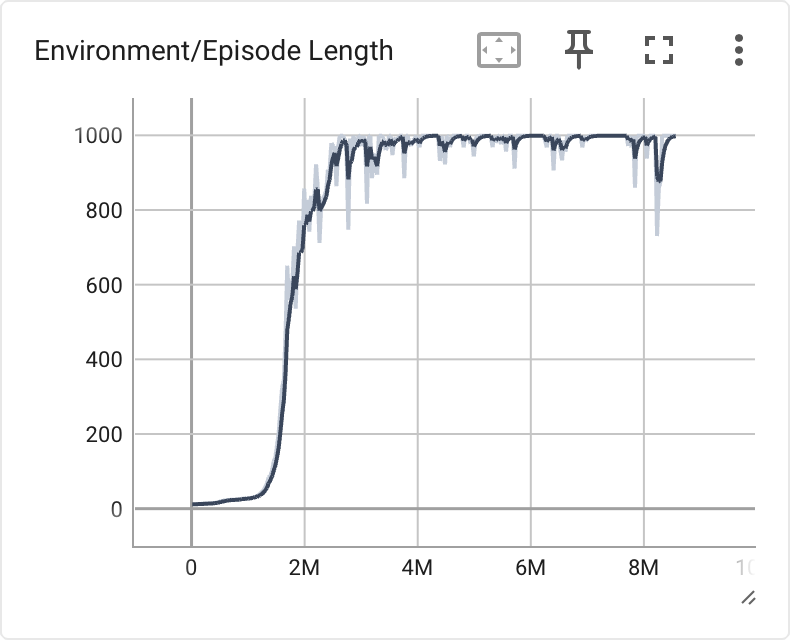
\includegraphics[width=\textwidth]{img/128_episode_length}
      \caption{Episodenlänge}
      \label{fig:128_episode_length}
    \end{subfigure}
    \begin{subfigure}{.49\textwidth}
      \centering  
      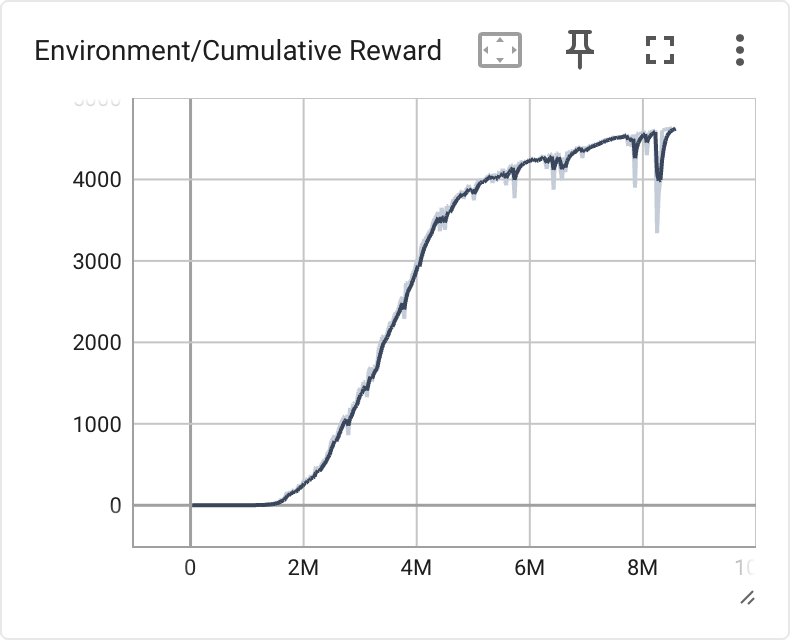
\includegraphics[width=\textwidth]{img/128_cumulative_reward}
      \caption{Angehäufte Belohnung}
      \label{fig:128_cumulative_reward}
    \end{subfigure}
     \begin{subfigure}{.49\textwidth}
      \centering  
      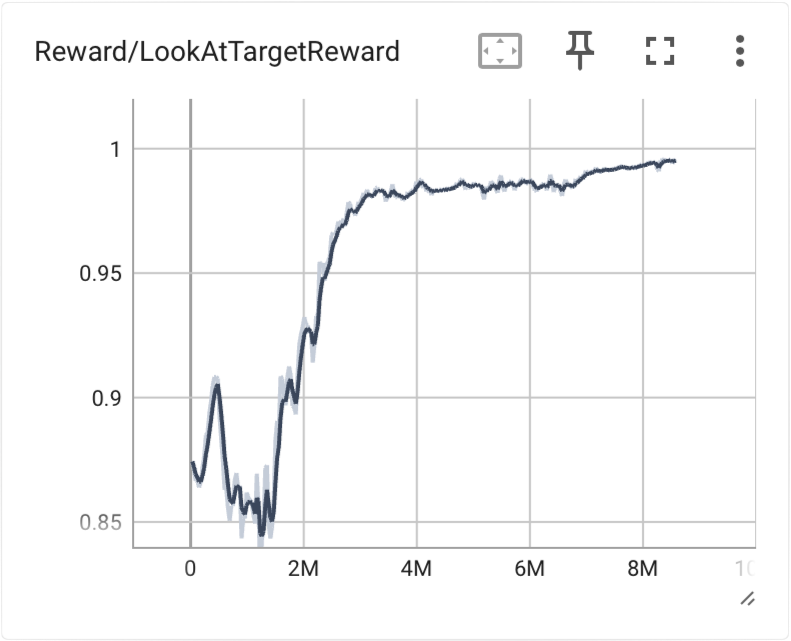
\includegraphics[width=\textwidth]{img/128_look_reward}
      \caption{Blickbelohnung}
      \label{fig:128_look_reward}
    \end{subfigure}
    \begin{subfigure}{.49\textwidth}
      \centering  
      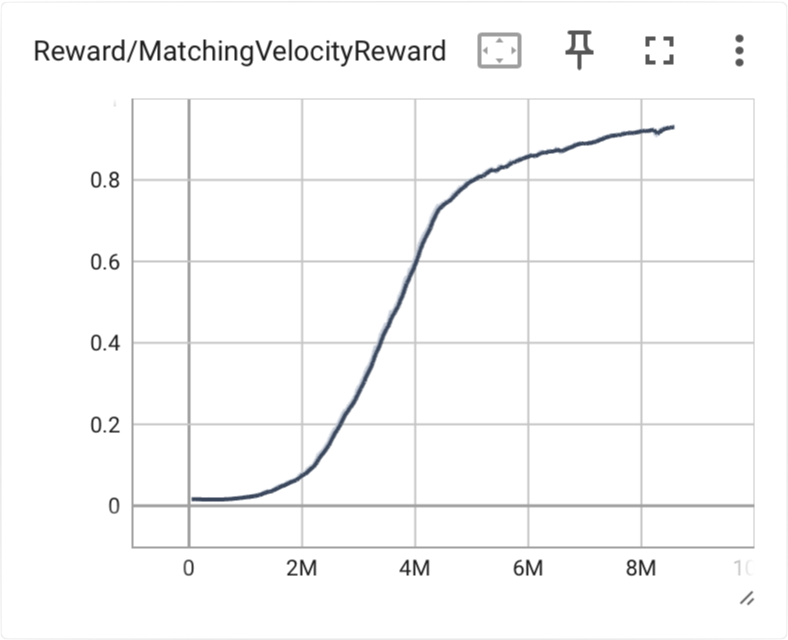
\includegraphics[width=\textwidth]{img/128_vel_reward}
      \caption{Geschwindigkeitsbelohnung}
      \label{fig:128_vel_reward}
    \end{subfigure}
    \begin{subfigure}{.49\textwidth}
      \centering  
      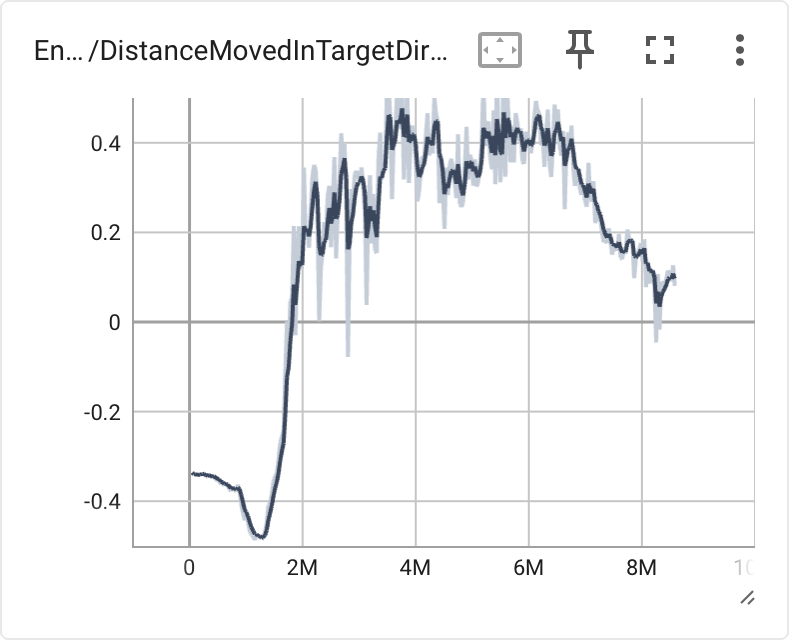
\includegraphics[width=\textwidth]{img/128_move_target_dir}
      \caption{Zurückgelegte Stecke in Zielrichtung}
      \label{fig:128_move_target_dir}
    \end{subfigure}
  \caption{Versuch 5 Training Graphen}
  \label{fig:versuch5_training}
\end{figure}

Nach dem erfolgreichen stehen auf einer festen Position, sind die nächsten Bewegungsziele die Bewegung zum Ziel mit unterschiedlichen Blickrichtungen. Die Extremfälle sind hier das Laufen rückwärts und seitwärts.
Im folgenden wird daher untersucht ob das Laufen in unterschiedliche Richtungen relativ zur Blickrichtung für den Läufer erlernbar ist. Um das zu realisieren wurde die Blickrichtung Belohnungsfunktion relativ zur Zielrichtung angepasst. Bei Vorwärtsbewegung ist die Blickrichtung gleich der Zielrichtung. Bei Seitlicherbewegung ist die Blickrichtung im rechten Winkel zur Zielrichtung. Bei der Rückwärtsbewegung ist die Blickrichtung entgegen der Zielrichtung. In \ref{lst:blickrichtung} ist die Implementierung für das bestimmen der Blickrichtung zu sehen.

\begin{lstlisting}[caption={Blickrichtung Enum und Belohnung},captionpos=b,label={lst:blickrichtung}]
public enum Direction
{
    Forward,
    Right,
    Left,
    Backward,
}
    
public override void FixedUpdate()
{
    ...
    var headForward = head.forward;
    headForward.y = 0;
    Vector3 lookDirection = cubeForward;
    switch (direction)
    {
        case Direction.Right:
            lookDirection = -walkOrientationCube.transform.right;
            break;
        case Direction.Left:
            lookDirection = walkOrientationCube.transform.right;
            break;
        case Direction.Backward:
            lookDirection = -walkOrientationCube.transform.forward;
            break;
    }
    var lookAtTargetReward = (Vector3.Dot(lookDirection, headForward) + 1) * 0.5F;
    ...
}
\end{lstlisting}

Das gehen in Zielrichtung wurde durch die Änderungen nicht beeinflusst. Separate Trainings zu den drei anderen Laufrichtungen waren erfolgreich. Abbildung \ref{fig:116_130_131_132_move_target_dir}, \ref{fig:116_130_131_132_reach_target} zeigen die zurückgelegte Distanz und die Anzahl an erreichten Zielen in einer Trainingsepisode. Die Ergebnisse der 3 Laufrichtungen sind alle vergleichbar mit den Ergebnissen der Demo. Die Abweichung der Laufrichtung Links ist vermutlich der zufällligen Natur des Trainings anzurechnen.

\begin{figure}[H]
  \centering  
  \begin{subfigure}{.49\textwidth}
      \centering  
      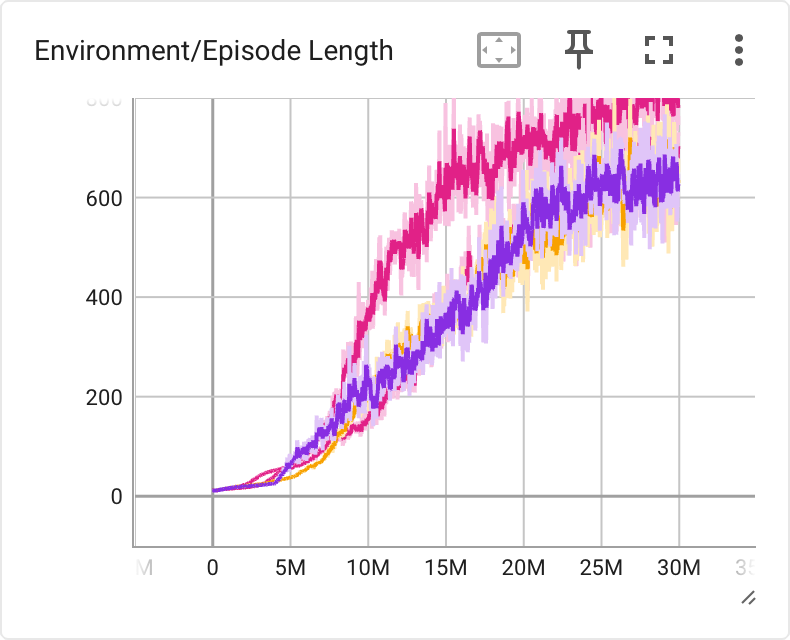
\includegraphics[width=\textwidth]{img/116_130_131_132_episode_length}
      \caption{Episodenlänge}
      \label{fig:116_130_131_132_episode_length}
    \end{subfigure}
    \begin{subfigure}{.49\textwidth}
      \centering  
      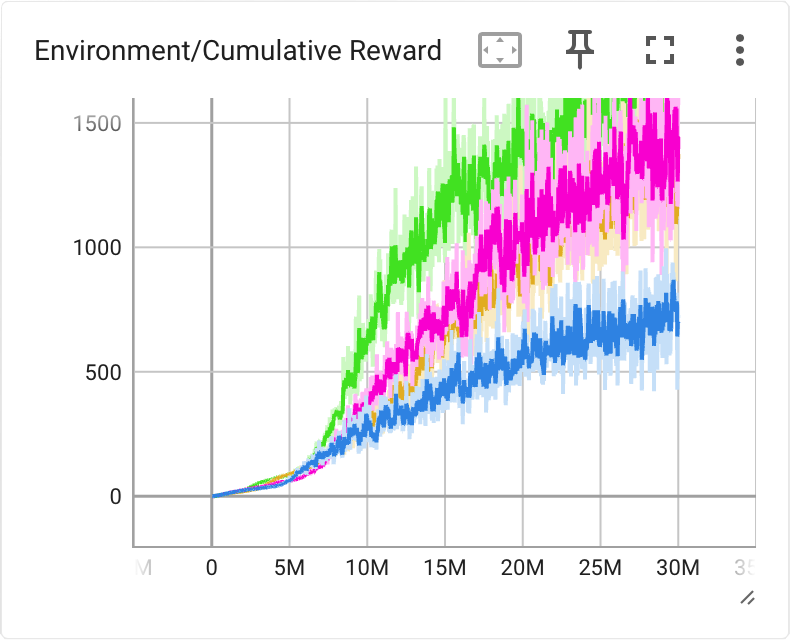
\includegraphics[width=\textwidth]{img/116_130_131_132_cumulative_reward}
      \caption{Angehäufte Belohnung}
      \label{fig:116_130_131_132_cumulative_reward}
    \end{subfigure}
     \begin{subfigure}{.49\textwidth}
      \centering  
      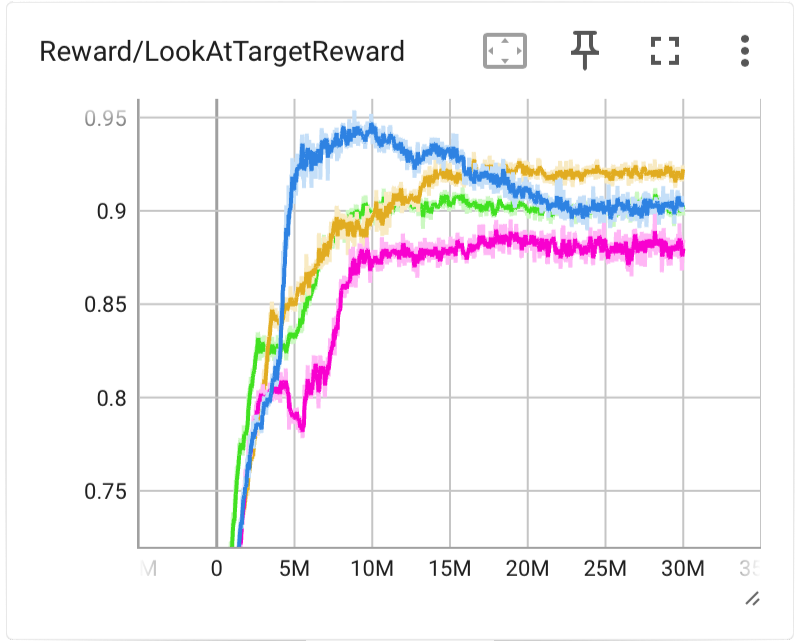
\includegraphics[width=\textwidth]{img/116_130_131_132_look_reward}
      \caption{Blickbelohnung}
      \label{fig:116_130_131_132_look_reward}
    \end{subfigure}
    \begin{subfigure}{.49\textwidth}
      \centering  
      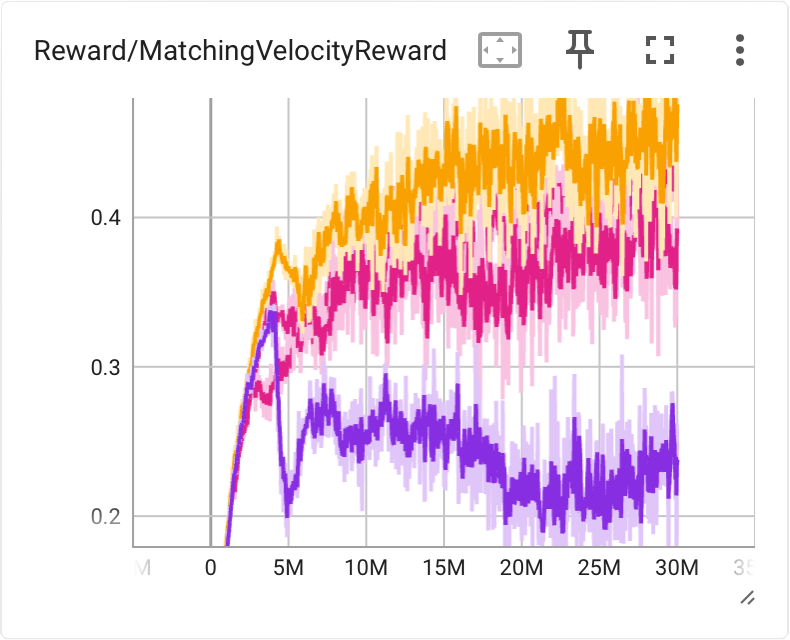
\includegraphics[width=\textwidth]{img/116_130_131_132_vel_reward}
      \caption{Geschwindigkeitsbelohnung}
      \label{fig:116_130_131_132_vel_reward}
    \end{subfigure}
    \begin{subfigure}{.49\textwidth}
      \centering  
      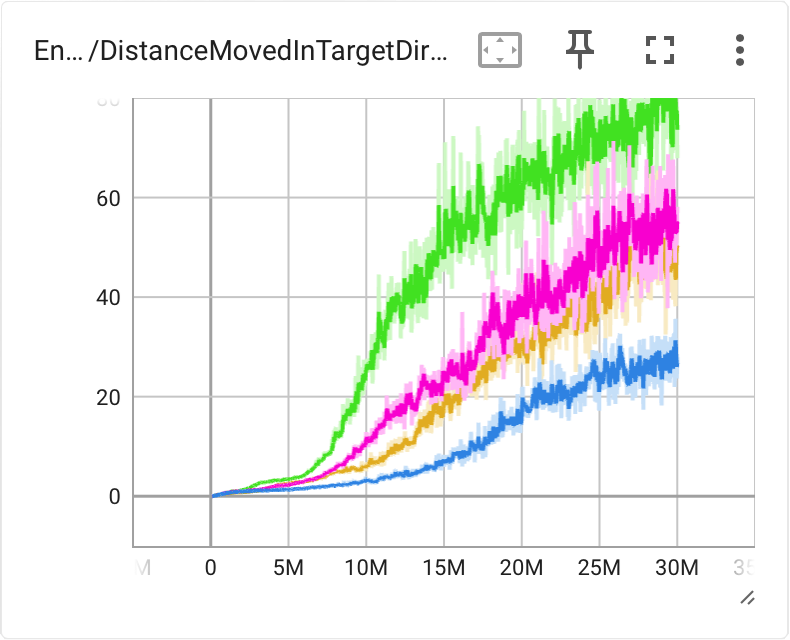
\includegraphics[width=\textwidth]{img/116_130_131_132_move_target_dir}
      \caption{Zurückgelegte Stecke in Zielrichtung}
      \label{fig:116_130_131_132_move_target_dir}
    \end{subfigure}
    \begin{subfigure}{.49\textwidth}
      \centering  
      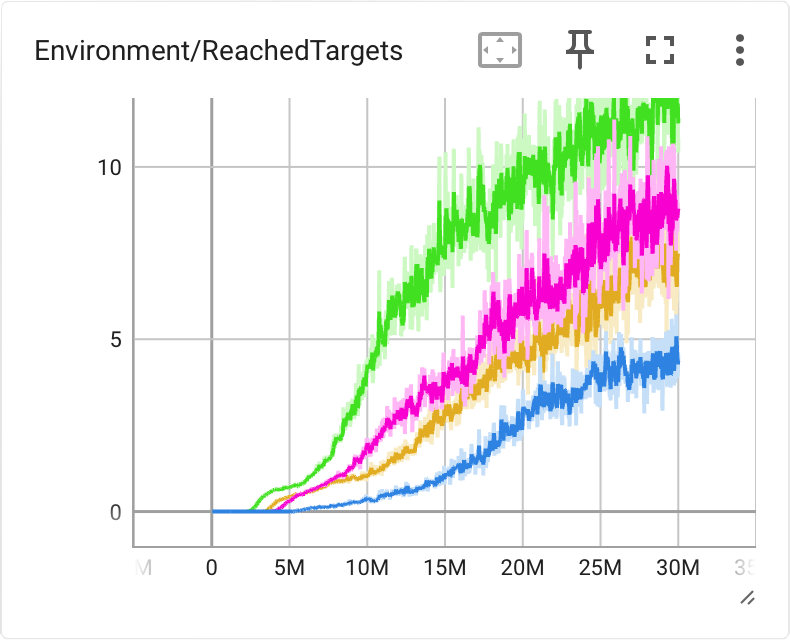
\includegraphics[width=\textwidth]{img/116_130_131_132_reach_target}
      \caption{Anzahl erreichte Ziele}
      \label{fig:116_130_131_132_reach_target}
    \end{subfigure}
  \caption{Unterschiedliche Blickrichtungen Training Graphen (grün = vorwärts, orange = rückwärts, rosa = rechts, blau = links)}
  \label{fig:training_unterschiedliche_blickrichtung}
\end{figure}